\begin{figure*}[t]
\centering
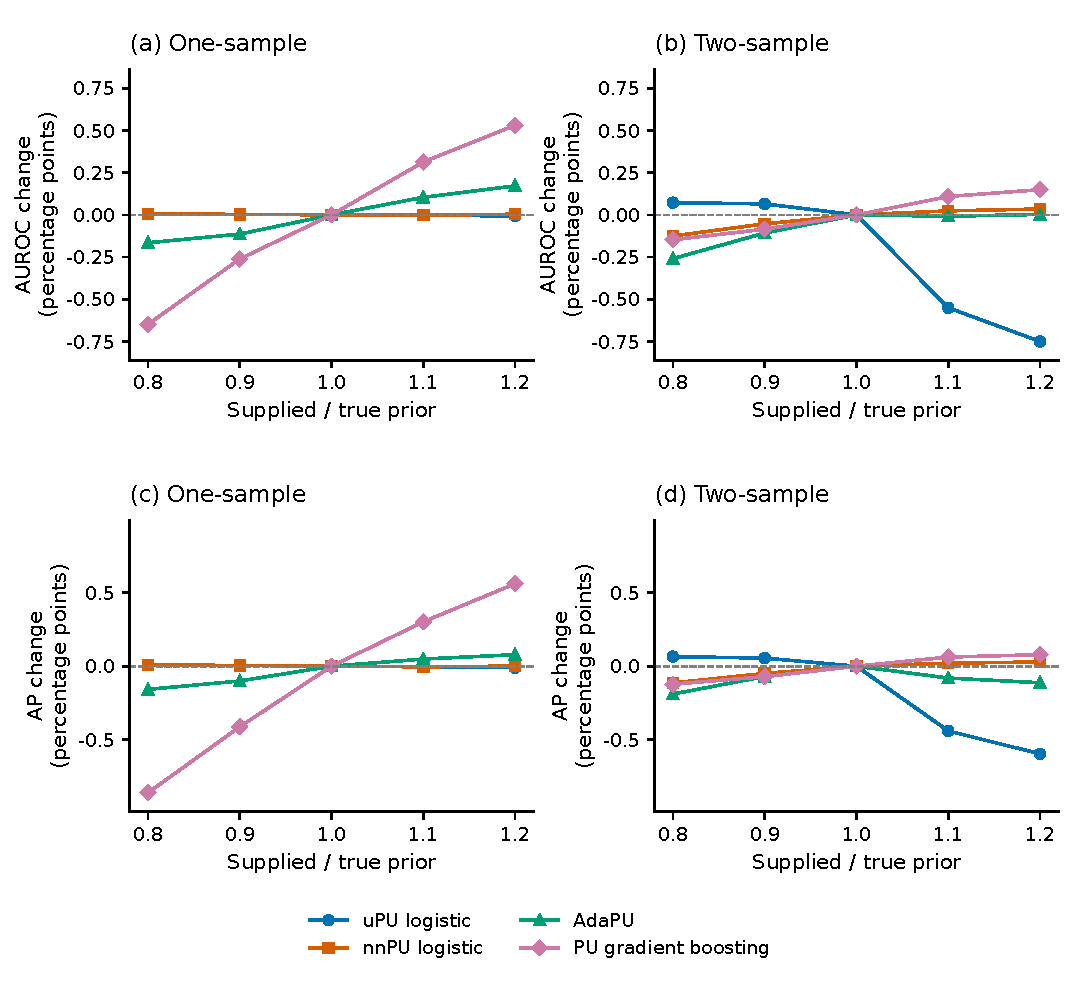
\includegraphics[page=1,width=\textwidth]{mlj_revision/display_package/supplement/figures/fig_s_supplied_prior_sensitivity.pdf}
\caption{Supplied-minus-correct-prior AUROC/AP changes for uPU logistic, nnPU logistic, AdaPU and PU gradient boosting. Eight prespecified settings are averaged equally; each setting has 100 paired repetitions. Table rows retain each setting and pointwise 95\% Monte Carlo intervals. The ratio-one point compares each archived correct-prior result with itself, so its difference is identically zero; it is not an imputation. One-sample labeling probability remains as in the archived sensitivity protocol. Equal-eight-setting supplied-prior sensitivity. Curves are equally weighted means of eight designed settings, not confidence bands or estimates over a random population of scenarios.}
\label{fig:fig-s-supplied-prior-sensitivity-page1}
\end{figure*}
